% vim: set ts=4 sw=4 tw=80 noexpandtab:

\documentclass{42-en}

%******************************************************************************%
%                                                                              %
%                                   Prologue                                   %
%                                                                              %
%******************************************************************************%
\usepackage[
    type={CC},
    modifier={by-nc-sa},
    version={4.0},
]{doclicense}

%****************************************************************%
%                  Re/definition of commands                     %
%****************************************************************%

\newcommand{\ailogo}[1]{\def \@ailogo {#1}}\ailogo{assets/42ai_logo.pdf}

%%  Redefine \maketitle
\makeatletter
\def \maketitle {
  \begin{titlepage}
    \begin{center}
	%\begin{figure}[t]
	  %\includegraphics[height=8cm]{\@ailogo}
	  
\includegraphics[height=8cm]{assets/42ai_logo.pdf}
	%\end{figure}
      \vskip 5em
      {\huge \@title}
      \vskip 2em
      {\LARGE \@subtitle}
      \vskip 4em
    \end{center}
    %\begin{center}
	  %\@author
    %\end{center}
	%\vskip 5em
  \vfill
  \begin{center}
    \emph{\summarytitle : \@summary}
  \end{center}
  \vspace{2cm}
  %\vskip 5em
  %\doclicenseThis
  \end{titlepage}
}
\makeatother

\makeatletter
\def \makeheaderfilesforbidden
{
  \noindent
  \begin{tabularx}{\textwidth}{|X X  X X|}
    \hline
  \multicolumn{1}{|>{\raggedright}m{1cm}|}
  {\vskip 2mm 
\includegraphics[height=1cm]{assets/42ai_logo.pdf}} &
  \multicolumn{2}{>{\centering}m{12cm}}{\small Exercise : \@exnumber } &
  \multicolumn{1}{ >{\raggedleft}p{1.5cm}|}
%%              {\scriptsize points : \@exscore} \\ \hline
              {} \\ \hline

  \multicolumn{4}{|>{\centering}m{15cm}|}
              {\small \@extitle} \\ \hline

  \multicolumn{4}{|>{\raggedright}m{15cm}|}
              {\small Turn-in directory : \ttfamily
                $ex\@exnumber/$ }
              \\ \hline
  \multicolumn{4}{|>{\raggedright}m{15cm}|}
              {\small Files to turn in : \ttfamily \@exfiles }
              \\ \hline

  \multicolumn{4}{|>{\raggedright}m{15cm}|}
              {\small Forbidden functions : \ttfamily \@exforbidden }
              \\ \hline

%%  \multicolumn{4}{|>{\raggedright}m{15cm}|}
%%              {\small Remarks : \ttfamily \@exnotes }
%%              \\ \hline
\end{tabularx}
%% \exnotes
\exrules
\exmake
\exauthorize{None}
\exforbidden{None}
\extitle{}
\exnumber{}
}
\makeatother

%%  Syntactic highlights
\makeatletter
\newenvironment{pythoncode}{%
  \VerbatimEnvironment
  \usemintedstyle{emacs}
  \minted@resetoptions
  \setkeys{minted@opt}{bgcolor=black,formatcom=\color{lightgrey},fontsize=\scriptsize}
  \begin{figure}[ht!]
    \centering
    \begin{minipage}{16cm}
      \begin{VerbatimOut}{\jobname.pyg}}
{%[
      \end{VerbatimOut}
      \minted@pygmentize{c}
      \DeleteFile{\jobname.pyg}
    \end{minipage}
\end{figure}}
\makeatother

\usemintedstyle{native}

\begin{document}

% =============================================================================%
%                     =====================================                    %

\title{Python \& ML - Module 04}
\subtitle{Pandas}
\author{
  Maxime Choulika (cmaxime), Pierre Peigné (ppeigne), Matthieu David (mdavid)
}

\summary
{
  Today you will learn how to use a Python library that will allow you
  to manipulate dataframes.
}
\maketitle
%******************************************************************************%
%                                                                              %
%                        Common Instructions                                   %
%                          for Python Projects                                 %
%                                                                              %
%******************************************************************************%

\chapter{Common Instructions}
\begin{itemize}
  \item The version of Python recommended to use is 3.7, you can
  check the version of Python with the following command: \texttt{python -V}
  
  \item The norm: during this piscine, it is recommended to follow the
  \href{https://www.python.org/dev/peps/pep-0008/}{PEP 8 standards}, though it is not mandatory.
  You can install \href{https://pypi.org/project/pycodestyle}{pycodestyle} which
  is a tool to check your Python code.
  
  \item The function \texttt{eval} is never allowed.
  
  \item The exercises are ordered from the easiest to the hardest.
  
  \item Your exercises are going to be evaluated by someone else,
  so make sure that your variable names and function names are appropriate and civil. 
  
  \item Your manual is the internet.
  
  \item You can also ask questions in the \texttt{\#bootcamps} channel in the \href{https://42-ai.slack.com}{42AI}
  or \href{42born2code.slack.com}{42born2code}.
  
  \item If you find any issue or mistakes in the subject please create an issue on \href{https://github.com/42-AI/bootcamp_python/issues}{42AI repository on Github}.  
  
  \item We encourage you to create test programs for your
  project even though this work \textbf{won't have to be
  submitted and won't be graded}. It will give you a chance
  to easily test your work and your peers’ work. You will find
  those tests especially useful during your defence. Indeed,
  during defence, you are free to use your tests and/or the
  tests of the peer you are evaluating.
  
  \item Submit your work to your assigned git repository. Only the work in the
  git repository will be graded. If Deepthought is assigned to grade your
  work, it will be run after your peer-evaluations.
  If an error happens in any section of your work during Deepthought's grading,
  the evaluation will stop.
\end{itemize}
\newpage
\tableofcontents
\startexercices

%                     =====================================                    %
% =============================================================================%


%******************************************************************************%
%                                                                              %
%                                   Exercises                                  %
%                                                                              %
%******************************************************************************%

% ============================================== %
% ===========================(start ex 00)       %
\chapter{Exercise 00}
\extitle{FileLoader}
\turnindir{ex00}
\exnumber{00}
\exfiles{FileLoader.py}
\exforbidden{None}
\makeheaderfilesforbidden

% ================================== %
\section*{Objective}
% ---------------------------------- %
The goal of this exercise is to create a Fileloader class containing a
load and a display method.

% ================================== %
\section*{Instructions}
% ---------------------------------- %
Write a class named \texttt{FileLoader} which implements the following methods:  
\begin{itemize}
  \item \texttt{load(self, path)}: takes as an argument the file path of the dataset to load, 
    displays a message specifying the dimensions of the dataset (e.g. 340 x 500) 
    and returns the dataset loaded as a pandas.DataFrame.
  \item \texttt{display(self, df, n)}: takes a pandas.DataFrame and an integer as arguments, 
    displays the first n rows of the dataset if n is positive, or the last n rows if n is negative.
\end{itemize}


\noindent \texttt{FileLoader} object should not raise any exceptions (wrong path, file does not exist, parameters different than a string ...).
% ================================== %
\section*{Examples}
% ---------------------------------- %
\begin{minted}[bgcolor=darcula-back,formatcom=\color{lightgrey},fontsize=\scriptsize]{python}
from FileLoader import FileLoader
loader = FileLoader()
data = loader.load("../data/adult_data.csv")
# Output
Loading dataset of dimensions 32561 x 15


loader.display(data, 12)
# Output
age         workclass  fnlwgt  ... hours-per-week  native-country salary
0    39         State-gov   77516  ...             40   United-States  <=50K
1    50  Self-emp-not-inc   83311  ...             13   United-States  <=50K
2    38           Private  215646  ...             40   United-States  <=50K
3    53           Private  234721  ...             40   United-States  <=50K
4    28           Private  338409  ...             40            Cuba  <=50K
5    37           Private  284582  ...             40   United-States  <=50K
6    49           Private  160187  ...             16         Jamaica  <=50K
7    52  Self-emp-not-inc  209642  ...             45   United-States   >50K
8    31           Private   45781  ...             50   United-States   >50K
9    42           Private  159449  ...             40   United-States   >50K
10   37           Private  280464  ...             80   United-States   >50K
11   30         State-gov  141297  ...             40           India   >50K

[12 rows x 15 columns]
\end{minted}

\hint{NB: Your terminal may display more columns if the window is wider.}

% ===========================(fin ex 00)         %
% ============================================== %
\newpage

% ============================================== %
% ===========================(start ex 01)       %
\chapter{Exercise 01}
\extitle{YoungestFellah}
\turnindir{ex01}
\exnumber{01}
\exfiles{FileLoader.py, YoungestFellah.py}
\exforbidden{None}
\makeheaderfilesforbidden


% ================================= %
\section*{Objective}
% --------------------------------- %
The goal of this exercise is to create a function that will return a
dictionary containing the age of the youngest woman and the youngest
man who took part in the Olympics a given year.

% ================================= %
\section*{Instructions}
% --------------------------------- %
This exercise uses the following dataset: \texttt{athlete\_events.csv}.

Write a function \texttt{youngest\_fellah} that takes two arguments:
\begin{itemize}
  \item a pandas.DataFrame which contains the dataset
  \item an Olympic year.
\end{itemize}

The function returns a dictionary containing the age of the youngest
woman and man who took part in the Olympics on that year.
The name of the dictionary's keys is up to you, but it must be self-explanatory.

% ================================= %
\section*{Examples}
% --------------------------------- %
\begin{minted}[bgcolor=darcula-back,formatcom=\color{lightgrey},fontsize=\scriptsize]{python}
from FileLoader import FileLoader
loader = FileLoader()
data = loader.load('../data/athlete_events.csv')
# Output
Loading dataset of dimensions 271116 x 15


from YoungestFellah import youngest_fellah
youngest_fellah(data, 2004)
# Output
{'f': 13.0, 'm': 14.0}
\end{minted}


% ===========================(fin ex 01)         %
% ============================================== %

\newpage

% ============================================== %
% ===========================(start ex 02)       %
\chapter{Exercise 02}
\extitle{ProportionBySport}
\turnindir{ex02}
\exnumber{02}
\exfiles{FileLoader.py, ProportionBySport.py}
\exforbidden{None}
\makeheaderfilesforbidden


% ================================= %
\section*{Objective}
% --------------------------------- %
The goal of this exercise is to create a function displaying
the proportion of participants who played a given sport, among
the participants of a given genders.

% ================================= %
\section*{Instructions}
% --------------------------------- %
This exercise uses the dataset \texttt{athlete\_events.csv}.

Write a function \texttt{proportion\_by\_sport} that takes four arguments:
\begin{itemize}
  \item a pandas.DataFrame of the dataset,
  \item an olympic year,
  \item a sport,
  \item a gender.
\end{itemize}

The function returns a float corresponding to the proportion (percentage) of participants 
who played the given sport among the participants of the given gender.

The function answers questions like the following : 
"What was the percentage of female basketball players among all the female 
participants of the 2016 Olympics?"


\hint{
Here and further, if needed, drop duplicated sports people
to count only unique ones. Beware to call the dropping function
at the right moment and with the right parameters, in order not to omit any individuals.
}

% ================================= %
\section*{Examples}
% --------------------------------- %
\begin{minted}[bgcolor=darcula-back,formatcom=\color{lightgrey},fontsize=\scriptsize]{python}
from FileLoader import FileLoader
loader = FileLoader()
data = loader.load('../data/athlete_events.csv')
# Output
Loading dataset of dimensions 271116 x 15


from ProportionBySport import proportion_by_sport
proportion_by_sport(data, 2004, 'Tennis', 'F')
# Output
0.01935634328358209
\end{minted}

We assume that we are always using appropriate arguments as input,
and thus do not need to handle input errors.

% ===========================(fin ex 02)         %
% ============================================== %

\newpage

% ============================================== %
% ===========================(start ex 03)       %
\chapter{Exercise 03}
\extitle{HowManyMedals}
\turnindir{ex03}
\exnumber{03}
\exfiles{FileLoader.py, HowManyMedals.py}
\exforbidden{None}
\makeheaderfilesforbidden


% ================================= %
\section*{Objective}
% --------------------------------- %
The goal of this exercise is to implement a function that will return
a dictionary of dictionaries giving the number and type of medals
for each year during which the participant won medals.

% ================================= %
\section*{Instructions}
% --------------------------------- %
This exercise uses the following dataset: \texttt{athlete\_events.csv}.


Write a function \texttt{how\_many\_medals} that takes two arguments:
\begin{itemize}
  \item a pandas.DataFrame which contains the dataset,
  \item a participant name.
\end{itemize}

The function returns a dictionary of dictionaries giving the number and type of medals 
for each year during which the participant won medals.
The keys of the main dictionary are the Olympic games years. 
In each year's dictionary, the keys are 'G', 'S', 'B' corresponding to the type of 
medals won (gold, silver, bronze). The innermost values correspond to the number of 
medals of a given type won for a given year.

% ================================= %
\section*{Examples}
% --------------------------------- %
\begin{minted}[bgcolor=darcula-back,formatcom=\color{lightgrey},fontsize=\scriptsize]{python}
from FileLoader import FileLoader
loader = FileLoader()
data = loader.load('../data/athlete_events.csv')
# Output
Loading dataset of dimensions 271116 x 15


from HowManyMedals import how_many_medals
how_many_medals(data, 'Kjetil Andr Aamodt')
# Output
{1992: {'G': 1, 'S': 0, 'B': 1},
 1994: {'G': 0, 'S': 2, 'B': 1},
 1998: {'G': 0, 'S': 0, 'B': 0},
 2002: {'G': 2, 'S': 0, 'B': 0},
 2006: {'G': 1, 'S': 0, 'B': 0}}
\end{minted}

% ===========================(fin ex 03)         %
% ============================================== %

\newpage

% ============================================== %
% ===========================(start ex 04)       %
\chapter{Exercise 04}
\extitle{SpatioTemporalData}
\turnindir{ex04}
\exnumber{04}
\exfiles{FileLoader.py, SpatioTemporalData.py}
\exforbidden{None}
\makeheaderfilesforbidden


% ================================= %
\section*{Objective}
% --------------------------------- %
The goal of this exercise is to implement a class called \texttt{SpatioTemporalData}
that takes a dataset (pandas.DataFrame) as argument in its constructor
and implements two methods.

% ================================= %
\section*{Instructions}
% --------------------------------- %
This exercise uses the dataset \texttt{athlete\_events.csv}.


Write a class called \texttt{SpatioTemporalData} that takes a dataset
(pandas.DataFrame) as argument in its constructor and implements the
following methods:
\begin{itemize}
  \item \texttt{when(location)}: takes a location as an argument and returns
        a list containing the years where games were held in the given location,  
  \item \texttt{where(date)}: takes a date as an argument and returns the location
        where the Olympics took place in the given year.
\end{itemize}

% ================================= %
\section*{Examples}
% --------------------------------- %
\begin{minted}[bgcolor=darcula-back,formatcom=\color{lightgrey},fontsize=\scriptsize]{python}
from FileLoader import FileLoader
loader = FileLoader()
data = loader.load('../data/athlete_events.csv')
# Output
Loading dataset of dimensions 271116 x 15


from SpatioTemporalData import SpatioTemporalData
sp = SpatioTemporalData(data)
sp.where(1896)
# Output
['Athina']


sp.where(2016)
# Output
['Rio de Janeiro']


sp.when('Athina')
# Output
[2004, 1906, 1896]


sp.when('Paris')
# Output
[1900, 1924]
\end{minted}


% ===========================(fin ex 04)         %
% ============================================== %

\newpage

% ============================================== %
% ===========================(start ex 05)       %
\chapter{Exercise 05}
\extitle{HowManyMedalsByCountry}
\turnindir{ex05}
\exnumber{05}
\exfiles{FileLoader.py, HowManyMedalsByCountry.py}
\exforbidden{None}
\makeheaderfilesforbidden


% ================================= %
\section*{Objective}
% --------------------------------- %
The goal of this exercise is to write a function that returns a
dictionary of dictionaries giving the number and type of medal for
each competition where the country delegation earned medals.

% ================================= %
\section*{Instructions}
% --------------------------------- %
This exercise uses the following dataset: \texttt{athlete\_events.csv}

Write a function \texttt{how\_many\_medals\_by\_country} that takes two arguments:
\begin{itemize}
  \item a pandas.DataFrame which contains the dataset  
  \item a country name.
\end{itemize}

The function returns a dictionary of dictionaries giving the number and
type of medal for each competition where the country delegation earned medals.  
The keys of the main dictionary are the Olympic games' years. In each
year's dictionary, the key are 'G', 'S', 'B' corresponding to the
type of medals won.

Duplicated medals per team games should be handled and not counted twice.
Hint: You may find this list to be of some use.
\begin{minted}[bgcolor=darcula-back,formatcom=\color{lightgrey},fontsize=\scriptsize]{python}
  team_sports = ['Basketball', 'Football',  'Tug-Of-War', 'Badminton', 'Sailing',
                 'Handball', 'Water Polo', 'Hockey', 'Rowing', 'Bobsleigh', 'Softball',
                 'Volleyball', 'Synchronized Swimming', 'Baseball', 'Rugby Sevens',
                 'Rugby', 'Lacrosse', 'Polo']
\end{minted}

% ================================= %
\section*{Examples}
% --------------------------------- %
\begin{minted}[bgcolor=darcula-back,formatcom=\color{lightgrey},fontsize=\scriptsize]{python}
from FileLoader import FileLoader
loader = FileLoader()
data = loader.load('../data/athlete_events.csv')
# Output
Loading dataset of dimensions 271116 x 15


from HowManyMedalsByCountry import how_many_medals_by_country
how_many_medals_by_country(data, 'Martian Federation')
# Output
{2192: {'G': 17, 'S': 14, 'B': 23}, 2196: {'G': 8, 'S': 21, 'B': 19}, 2200: {'G': 26, 'S': 19, 'B': 7}}
\end{minted}

You probably guessed by now that we gave up providing real examples...

If you want real examples, you can easily look online.
Do beware that some medals might be awarded or removed years after the games
are over, for example if a previous medallist was found to have cheated
and is sanctioned.
The \texttt{athlete\_events.csv} dataset might not always take these posterior
changes into account.

% ===========================(fin ex 05)         %
% ============================================== %

\newpage

% ============================================== %
% ===========================(start ex 06)       %
\chapter{Exercise 06}
\extitle{MyPlotLib}
\turnindir{ex06}
\exnumber{06}
\exfiles{MyPlotLib.py}
\exforbidden{None}
\makeheaderfilesforbidden


% ================================= %
\section*{Objective}
% --------------------------------- %
The goal the exercise is to introduce plotting methods among the different
libraries Pandas, Matplotlib, Seaborn or Scipy.

% ================================= %
\section*{Instructions}
% --------------------------------- %
This exercise uses the following dataset: \texttt{athlete\_events.csv}

Write a class called \texttt{MyPlotLib}. This class implements different plotting
methods, each of which take two arguments:
\begin{itemize}
  \item a pandas.DataFrame which contains the dataset,
  \item a list of feature names.
\end{itemize}

\hint{
  What is a feature? https://towardsdatascience.com/feature-engineering-for-machine-learning-3a5e293a5114
}

\begin{itemize}
  \item \texttt{histogram(data, features)}: plots one histogram for each numerical feature in the list,
  \item \texttt{density(data, features)}: plots the density curve of each numerical feature in the list,
  \item \texttt{pair\_plot(data, features)}: plots a matrix of subplots (also called scatter plot matrix).
        On each subplot shows a scatter plot of one numerical variable against another one.
        The main diagonal of this matrix shows simple histograms.
  \item \texttt{box\_plot(data, features)}: displays a box plot for each numerical variable in the dataset.
\end{itemize}

% ================================= %
\section*{Examples}
% --------------------------------- %

\begin{figure}[h!]
  \begin{minipage}[l]{0.49\linewidth}
    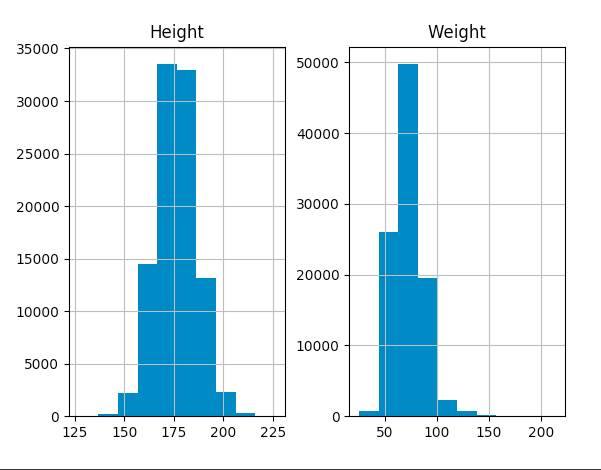
\includegraphics[scale=0.39]{assets/ex06_histogram.png}
    \caption{histogram}
  \end{minipage}
  \hfill
  \begin{minipage}[c]{0.49\linewidth}
    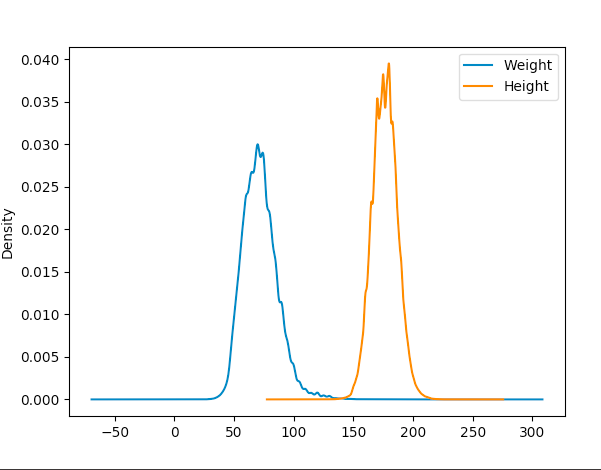
\includegraphics[scale=0.39]{assets/ex06_density.png}
    \caption{density}
  \end{minipage}
  
  \begin{minipage}[l]{0.49\linewidth}
    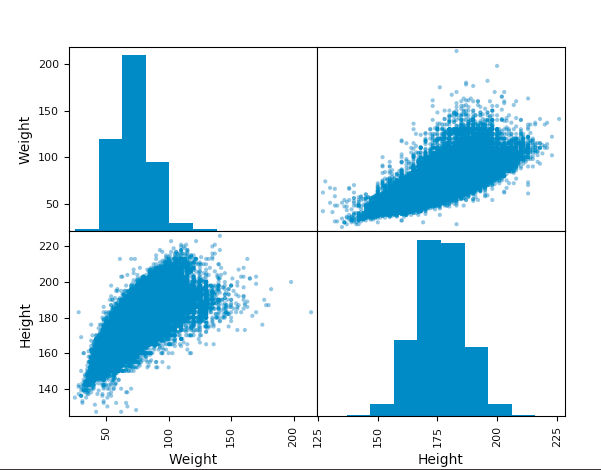
\includegraphics[scale=0.39]{assets/ex06_pair_plot.png}
    \caption{pair plot}
  \end{minipage}
  \hfill
  \begin{minipage}[c]{0.49\linewidth}
    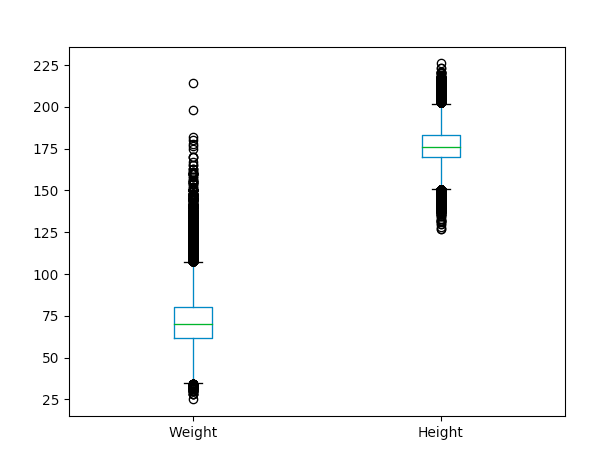
\includegraphics[scale=0.39]{assets/ex06_box_plot.png}
    \caption{box plot}
  \end{minipage}  
\end{figure}


% ===========================(fin ex 06)         %
% ============================================== %

\newpage

% ============================================== %
% ===========================(start ex 07)       %
\chapter{Exercise 07}
\extitle{Komparator}
\turnindir{ex07}
\exnumber{07}
\exfiles{Komparator.py, MyPlotLib.py (optional)}
\exforbidden{None}
\makeheaderfilesforbidden


% ================================= %
\section*{Objective}
% --------------------------------- %
The goal the exercise is to introduce plotting methods among the different
libraries Pandas, Matplotlib, Seaborn or Scipy.

% ================================= %
\section*{Instructions}
% --------------------------------- %
This exercise uses the following dataset: \texttt{athlete\_events.csv}.


Write a class called \texttt{Komparator} whose constructor takes as an argument a pandas.DataFrame which contains the dataset.
The class must implement the following methods, which take as input two variable names:
\begin{itemize}
  \item \texttt{compare\_box\_plots(self, categorical\_var, numerical\_var)}: displays a series of box plots 
  to compare how the distribution of the numerical variable changes if we only consider 
  the subpopulation which belongs to each category. 
  There should be as many box plots as categories. 
  For example, with Sex and Height, we would compare 
  the height distributions of men vs. women with two box plots.
  \item \texttt{density(self, categorical\_var, numerical\_var)}: displays the density of the numerical variable.
  Each subpopulation should be represented by a separate curve on the graph.
  \item \texttt{compare\_histograms(self, categorical\_var, numerical\_var)}: plots the numerical variable in a separate histogram for each category.
  As an extra, you can use overlapping histograms with a color code.
\end{itemize}

BONUS: Your functions can also accept a list of numerical variables (instead of just one), and output a comparison plot for each variable in the list.

% ===========================(fin ex 07)         %
% ============================================== %

\newpage

% ================================= %
\section*{Contact}
% --------------------------------- %
You can contact 42AI association by email: contact@42ai.fr\\
You can join the association on \href{https://join.slack.com/t/42-ai/shared_invite/zt-ebccw5r7-YPkDM6xOiYRPjqJXkrKgcA}{42AI slack}
and/or posutale to \href{https://forms.gle/VAFuREWaLmaqZw2D8}{one of the association teams}.

% ================================= %
\section*{Acknowledgements}
% --------------------------------- %
The modules Python \& ML is the result of a collective work, we would like to thanks:
\begin{itemize}
  \item Maxime Choulika (cmaxime),
  \item Pierre Peigné (ppeigne),
  \item Matthieu David (mdavid).
\end{itemize}
who supervised the creation, the enhancement and this present transcription.

\begin{itemize}
    \item Amric Trudel (amric@42ai.fr)
    \item Baptiste Lefeuvre (blefeuvr@student.42.fr)
    \item Mathilde Boivin (mboivin@student.42.fr)
    \item Tristan Duquesne (tduquesn@student.42.fr)
    \item Quentin Feuillade Montixi (qfeuilla@student.42.fr)
\end{itemize}
for your investment for the creation and development of these modules.

\begin{itemize}
    \item Barthélémy Leveque (bleveque@student.42.fr)
    \item Remy Oster (roster@student.42.fr)
    \item Quentin Bragard (qbragard@student.42.fr)
    \item Marie Dufourq (madufour@student.42.fr)
    \item Adrien Vardon (advardon@student.42.fr)
\end{itemize}
who betatest the first version of the modules of Machine Learning.
\vfill
\doclicenseThis

\end{document}